\begin{table}[t]
%\vspace{-50pt}
 \centering
\caption{Mean Geographic Origin Association by Speaker Language and Child Grade}
\begin{footnotesize}
\renewcommand{\tabcolsep}{0.15cm}
\label{tab:geographic-origins-means}
\begin{tabular}{p{.1in}lrrrrrrrrr}
\toprule
 &  & \multicolumn{3}{c}{3rd} & \multicolumn{3}{c}{5th} & \multicolumn{3}{c}{7th} \\
\cline{3-5} \cline{6-8} \cline{9-11}
&  & \textit{n} & \textit{M} & [95\% \textit{CI}] &  \textit{n} & \textit{M} & [95\% \textit{CI}] &  \textit{n}  & \textit{M} & [95\% \textit{CI}]\\
\midrule
\multicolumn{11}{l}{\textbf{Gujarat (Same State as Me)}}\\
 & Gujarati & 17 & 0.44 & [0.28, 0.6] & 72 & 0.74 & [0.65, 0.82] & 72 & 0.77 & [0.69, 0.85]\\

 & Hindi & 31 & 0.79 & [0.66, 0.92] & 48 & 0.49 & [0.4, 0.59] & 63 & 0.68 & [0.59, 0.77]\\

 & Urdu & 26 & 0.68 & [0.53, 0.84] & 49 & 0.51 & [0.4, 0.61] & 55 & 0.59 & [0.48, 0.68]\\

 & Marathi & 16 & 0.41 & [0.26, 0.56] & 28 & 0.29 & [0.2, 0.38] & 31 & 0.33 & [0.25, 0.43]\\

 & Tamil & 12 & 0.31 & [0.17, 0.45] & 15 & 0.15 & [0.08, 0.24] & 6 & 0.06 & [0.02, 0.12]\\

 & English (India) & 12 & 0.32 & [0.17, 0.47] & 10 & 0.10 & [0.04, 0.17] & 10 & 0.11 & [0.05, 0.17]\\

 & English (U.S.) & 11 & 0.28 & [0.15, 0.43] & 5 & 0.05 & [0.01, 0.1] & 8 & 0.08 & [0.03, 0.15]\\

& Mandarin & 4 & 0.10 & [0.02, 0.21] & 4 & 0.04 & [0.01, 0.08] & 1 & 0.01 & [0, 0.03]\\

\midrule
\multicolumn{11}{l}{\textbf{India (Different State)}}\\
  & Gujarati & 8 & 0.21 & [0.08, 0.35] & 16 & 0.16 & [0.1, 0.24] & 14 & 0.15 & [0.09, 0.23]\\

 & Hindi & 3 & 0.08 & [0, 0.17] & 46 & 0.47 & [0.38, 0.57] & 29 & 0.31 & [0.22, 0.41]\\

 & Urdu & 8 & 0.21 & [0.1, 0.34] & 42 & 0.43 & [0.33, 0.54] & 33 & 0.35 & [0.26, 0.46]\\

 & Marathi & 13 & 0.33 & [0.19, 0.49] & 54 & 0.56 & [0.46, 0.65] & 56 & 0.60 & [0.5, 0.71]\\

 & Tamil & 17 & 0.44 & [0.29, 0.59] & 51 & 0.53 & [0.43, 0.63] & 67 & 0.71 & [0.62, 0.8]\\

 & English (India) & 6 & 0.16 & [0.05, 0.28] & 18 & 0.19 & [0.11, 0.27] & 19 & 0.20 & [0.13, 0.29]\\

 & English (U.S.) & 11 & 0.28 & [0.14, 0.43] & 25 & 0.26 & [0.18, 0.35] & 14 & 0.15 & [0.08, 0.22]\\

& Mandarin & 7 & 0.18 & [0.07, 0.32] & 19 & 0.20 & [0.12, 0.28] & 19 & 0.20 & [0.13, 0.28]\\

\midrule
\multicolumn{11}{l}{\textbf{Foreign (Outside India)}}\\
& Gujarati & 13 & 0.33 & [0.19, 0.49] & 9 & 0.09 & [0.04, 0.15] & 7 & 0.08 & [0.02, 0.13]\\

 & Hindi & 5 & 0.13 & [0.03, 0.24] & 2 & 0.02 & [0, 0.05] & 0 & --- & ---\\

 & Urdu & 3 & 0.08 & [0, 0.18] & 4 & 0.04 & [0.01, 0.08] & 4 & 0.04 & [0.01, 0.09]\\

 & Marathi & 9 & 0.23 & [0.1, 0.38] & 14 & 0.14 & [0.08, 0.22] & 4 & 0.04 & [0.01, 0.09]\\

 & Tamil & 10 & 0.26 & [0.12, 0.38] & 30 & 0.31 & [0.21, 0.4] & 14 & 0.15 & [0.09, 0.22]\\

 & English (India) & 18 & 0.47 & [0.32, 0.63] & 68 & 0.71 & [0.61, 0.8] & 63 & 0.67 & [0.59, 0.77]\\

 & English (U.S.) & 16 & 0.41 & [0.27, 0.56] & 65 & 0.67 & [0.58, 0.77] & 70 & 0.74 & [0.64, 0.82]\\

& Mandarin & 25 & 0.64 & [0.47, 0.79] & 71 & 0.73 & [0.64, 0.82] & 70 & 0.75 & [0.67, 0.83]\\

\midrule
\multicolumn{11}{l}{\textbf{No Opinion}}\\
& Gujarati & 1 & 0.03 & [0, 0.08] & 0 & --- & --- & 0 & --- & ---\\

 & Hindi & 0 & --- & --- & 1 & 0.01 & [0, 0.03] & 1 & 0.01 & [0, 0.03]\\

 & Urdu & 1 & 0.03 & [0, 0.09] & 2 & 0.02 & [0, 0.05] & 2 & 0.02 & [0, 0.05]\\

 & Marathi & 1 & 0.03 & [0, 0.08] & 1 & 0.01 & [0, 0.03] & 2 & 0.02 & [0, 0.05]\\

 & Tamil & 0 & --- & --- & 1 & 0.01 & [0, 0.03] & 7 & 0.07 & [0.03, 0.13]\\

 & English (India) & 2 & 0.05 & [0, 0.14] & 0 & --- & --- & 2 & 0.02 & [0, 0.05]\\

 & English (U.S.) & 1 & 0.03 & [0, 0.08] & 2 & 0.02 & [0, 0.05] & 3 & 0.03 & [0, 0.07]\\

& Mandarin & 3 & 0.08 & [0, 0.17] & 3 & 0.03 & [0, 0.07] & 3 & 0.03 & [0, 0.08]\\
\bottomrule
\end{tabular}
\end{footnotesize}
\end{table}

\thispagestyle{empty}
\begin{table}[H]
\vspace{-20pt}
\centering
\caption{Mean Religious Association by Speaker Language and Child Grade}\label{tab:religion-means}\\
\begin{footnotesize}
%\renewcommand{\tabcolsep}{0.15cm}
\begin{tabular}{p{.1in}lrrrrrrrrr}
%\begin{tabular}{p{.1in}lrrrrrrrrr}
\toprule
 &  & \multicolumn{3}{c}{\textbf{3rd}} & \multicolumn{3}{c}{\textbf{5th}} & \multicolumn{3}{c}{\textbf{7th}} \\
\cline{3-5} \cline{6-8} \cline{9-11}\\[-.75em]
&  & \textit{n} & \textit{M} & [95\% \textit{CI}] &  \textit{n} & \textit{M} & [95\% \textit{CI}] &  \textit{n}  & \textit{M} & [95\% \textit{CI}]\\
\midrule
\multicolumn{11}{l}{\textbf{Hindu}}\\
 & Gujarati & 12 & 0.32 & [0.18, 0.49] & 72 & 0.71 & [0.61, 0.79] & 67 & 0.71 & [0.62, 0.80]\\

 & Hindi & 11 & 0.29 & [0.14, 0.43] & 54 & 0.53 & [0.45, 0.63] & 50 & 0.53 & [0.44, 0.63]\\

 & Urdu & 12 & 0.33 & [0.19, 0.48] & 46 & 0.46 & [0.36, 0.55] & 44 & 0.47 & [0.38, 0.57]\\

 & Marathi & 7 & 0.18 & [0.07, 0.32] & 48 & 0.48 & [0.38, 0.57] & 56 & 0.60 & [0.50, 0.69]\\

 & Tamil & 9 & 0.24 & [0.12, 0.38] & 17 & 0.17 & [0.10, 0.25] & 10 & 0.11 & [0.05, 0.17]\\

 & English (India) & 10 & 0.27 & [0.14, 0.42] & 15 & 0.15 & [0.08, 0.23] & 9 & 0.10 & [0.04, 0.16]\\

 & English (U.S.) & 8 & 0.21 & [0.08, 0.35] & 5 & 0.05 & [0.01, 0.09] & 7 & 0.07 & [0.02, 0.13]\\

& Mandarin & 4 & 0.11 & [0.02, 0.21] & 3 & 0.03 & [0.00, 0.07] & 0 & --- & ---\\

\midrule
\multicolumn{11}{l}{\textbf{Muslim}}\\
 & Gujarati & 10 & 0.27 & [0.14, 0.41] & 7 & 0.07 & [0.03, 0.12] & 11 & 0.12 & [0.05, 0.18]\\

 & Hindi & 19 & 0.50 & [0.33, 0.66] & 34 & 0.34 & [0.25, 0.43] & 26 & 0.28 & [0.19, 0.36]\\

 & Urdu & 21 & 0.58 & [0.42, 0.74] & 40 & 0.40 & 0.30, 0.49] & 39 & 0.42 & [0.32, 0.53]\\

 & Marathi & 9 & 0.24 & [0.11, 0.37] & 10 & 0.10 & [0.05, 0.16] & 1 & 0.01 & [0.00, 0.03]\\

 & Tamil & 9 & 0.24 & [0.10, 0.37] & 11 & 0.11 & [0.05, 0.18] & 6 & 0.06 & [0.02, 0.12]\\

 & English (India) & 5 & 0.14 & [0.03, 0.26] & 12 & 0.12 & [0.06, 0.19] & 1 & 0.01 & [0.00, 0.03]\\

 & English (U.S.) & 4 & 0.11 & [0.03, 0.21] & 13 & 0.13 & [0.07, 0.20] & 3 & 0.03 & [0.00, 0.07]\\
 & Mandarin & 4 & 0.11 & [0.02, 0.21] & 9 & 0.09 & [0.04, 0.15] & 6 & 0.06 & [0.02, 0.12]\\
 \midrule
\multicolumn{11}{l}{\textbf{Jain}}\\
  & Gujarati & 7 & 0.19 & [0.08, 0.32] & 10 & 0.10 & [0.05, 0.16] & 3 & 0.03 & [0.00, 0.06]\\

 & Hindi & 4 & 0.11 & [0.02, 0.21] & 8 & 0.08 & [0.03, 0.14] & 9 & 0.10 & [0.04, 0.15]\\

 & Urdu & 0 & --- & --- & 10 & 0.10 & [0.04, 0.16] & 3 & 0.03 & [0.00, 0.07]\\

 & Marathi & 8 & 0.21 & [0.09, 0.34] & 16 & 0.16 & [0.09, 0.23] & 5 & 0.05 & [0.02, 0.11]\\

 & Tamil & 7 & 0.18 & [0.06, 0.31] & 30 & 0.30 & [0.22, 0.39] & 18 & 0.19 & [0.12, 0.27]\\

 & English (India) & 6 & 0.16 & [0.05, 0.30] & 16 & 0.16 & [0.10, 0.23] & 6 & 0.07 & [0.02, 0.12]\\

 & English (U.S.) & 5 & 0.13 & [0.03, 0.24] & 20 & 0.20 & [0.12, 0.28] & 5 & 0.05 & [0.01, 0.09]\\

& Mandarin & 7 & 0.18 & [0.07, 0.31] & 18 & 0.18 & [0.11, 0.26] & 12 & 0.13 & [0.07, 0.20]\\
 \midrule
\multicolumn{11}{l}{\textbf{Christian}}\\
 & Gujarati & 5 & 0.14 & [0.03, 0.26] & 4 & 0.04 & [0.01, 0.08] & 3 & 0.03 & [0.00, 0.07]\\

 & Hindi & 0 & --- & --- & 4 & 0.04 & [0.01, 0.08] & 1 & 0.01 & [0.00, 0.03]\\

 & Urdu & 4 & 0.11 & [0.02, 0.22] & 3 & 0.03 & [0.00, 0.07] & 0 & --- & ---\\

 & Marathi & 6 & 0.16 & [0.05, 0.28] & 8 & 0.08 & [0.03, 0.14] & 4 & 0.04 & [0.01, 0.09]\\

 & Tamil & 8 & 0.21 & [0.08, 0.35] & 16 & 0.16 & [0.09, 0.24] & 5 & 0.05 & [0.01, 0.11]\\

 & English (India) & 12 & 0.32 & [0.18, 0.48] & 32 & 0.32 & [0.24, 0.41] & 48 & 0.52 & [0.42, 0.62]\\

 & English (U.S.) & 14 & 0.37 & [0.22, 0.52] & 36 & 0.36 & [0.27, 0.46] & 40 & 0.42 & [0.33, 0.52]\\
& Mandarin & 10 & 0.26 & [0.14, 0.41] & 20 & 0.20 & [0.13, 0.28] & 21 & 0.23 & [0.15, 0.31]\\
 \midrule
\multicolumn{11}{l}{\textbf{Buddhist}}\\
& Gujarati & 3 & 0.08 & [0.00, 0.18] & 4 & 0.04 & [0.01, 0.08] & 3 & 0.03 & [0.00, 0.07]\\

 & Hindi & 3 & 0.08 & [0.00, 0.18] & 0 & --- & --- & 2 & 0.02 & [0.00, 0.05]\\

 & Urdu & 0 & --- & --- & 1 & 0.01 & [0.00, 0.03] & 3 & 0.03 & [0.00, 0.07]\\

 & Marathi & 5 & 0.13 & [0.05, 0.25] & 10 & 0.10 & [0.05, 0.16] & 14 & 0.15 & [0.07, 0.22]\\

 & Tamil & 2 & 0.05 & [0.00, 0.13] & 18 & 0.18 & [0.11, 0.25] & 31 & 0.33 & [0.23, 0.43]\\

 & English (India) & 1 & 0.03 & [0.00, 0.09] & 7 & 0.07 & [0.03, 0.13] & 4 & 0.04 & [0.01, 0.09]\\

 & English (U.S.) & 4 & 0.11 & [0.02, 0.21] & 10 & 0.10 & [0.05, 0.16] & 8 & 0.08 & [0.03, 0.15]\\

& Mandarin & 5 & 0.13 & [0.03, 0.24] & 16 & 0.16 & [0.09, 0.23] & 9 & 0.10 & [0.04, 0.16]\\
 \midrule
\multicolumn{11}{l}{\textbf{No Opinion}}\\
& Gujarati & 0 & --- & --- & 4 & 0.04 & [0.01, 0.08] & 7 & 0.07 & [0.02, 0.14]\\

 & Hindi & 1 & 0.03 & [0.00, 0.08] & 1 & 0.01 & [0.00, 0.03] & 6 & 0.06 & [0.02, 0.12]\\

 & Urdu & 0 & --- & --- & 1 & 0.01 & [0.00, 0.03] & 5 & 0.05 & [0.01, 0.11]\\

 & Marathi & 3 & 0.08 & [0.00, 0.17] & 9 & 0.09 & [0.04, 0.15] & 14 & 0.15 & [0.07, 0.22]\\

 & Tamil & 3 & 0.08 & [0.00, 0.18] & 9 & 0.09 & [0.04, 0.15] & 25 & 0.27 & [0.18, 0.35]\\

 & English (India) & 3 & 0.08 & [0.00, 0.18] & 18 & 0.18 & [0.11, 0.26] & 24 & 0.26 & [0.18, 0.35]\\

 & English (U.S.) & 3 & 0.08 & [0.00, 0.17] & 17 & 0.17 & [0.10, 0.24] & 32 & 0.34 & [0.24, 0.43]\\

& Mandarin & 8 & 0.21 & [0.09, 0.35] & 35 & 0.35 & [0.25, 0.45] & 45 & 0.48 & [0.38, 0.59]\\

\bottomrule
%\end{tabular}
\end{tabular}
\end{footnotesize}
\end{table}
\begin{table}[t]
\centering
\caption{Mean Wealth Association by Speaker Language and Child Grade}\\
\begin{footnotesize}
\label{tab:wealth-means}
\begin{tabular}{p{.1in}lrrrrrrrrr}
\toprule
 &  & \multicolumn{3}{c}{\textbf{3rd}} & \multicolumn{3}{c}{\textbf{5th}} & \multicolumn{3}{c}{\textbf{7th}} \\
\cline{3-5} \cline{6-8} \cline{9-11}\\[-.75em]
&  & \textit{n} & \textit{M} & [95\% \textit{CI}] &  \textit{n} & \textit{M} & [95\% \textit{CI}] &  \textit{n}  & \textit{M} & [95\% \textit{CI}]\\
\midrule
\multicolumn{11}{l}{\textbf{Less Money}}\\
 & Gujarati & 5 & 0.13 & [0.03, 0.25] & 24 & 0.24 & [0.16, 0.32] & 12 & 0.13 & [0.07, 0.20]\\

 & Hindi & 9 & 0.24 & [0.12, 0.39] & 22 & 0.22 & [0.14, 0.31] & 12 & 0.13 & [0.06, 0.20]\\

 & Urdu & 7 & 0.18 & [0.07, 0.31] & 16 & 0.16 & [0.09, 0.23] & 8 & 0.09 & [0.03, 0.15]\\

 & Marathi & 6 & 0.17 & [0.05, 0.30] & 23 & 0.23 & [0.15, 0.31] & 8 & 0.09 & [0.03, 0.15]\\

 & Tamil & 6 & 0.16 & [0.05, 0.29] & 25 & 0.25 & [0.17, 0.33] & 18 & 0.19 & [0.12, 0.28]\\

 & English (India) & 8 & 0.22 & [0.09, 0.35] & 13 & 0.13 & [0.07, 0.20] & 10 & 0.11 & [0.05, 0.18]\\

 & English (U.S.) & 5 & 0.13 & [0.05, 0.24] & 9 & 0.09 & [0.04, 0.15] & 6 & 0.06 & [0.02, 0.12]\\

& Mandarin & 4 & 0.11 & [0.02, 0.21] & 8 & 0.08 & [0.03, 0.13] & 12 & 0.13 & [0.06, 0.19]\\
\midrule
\multicolumn{11}{l}{\textbf{As Much Money}}\\
 & Gujarati & 13 & 0.34 & [0.20, 0.5] & 43 & 0.43 & [0.33, 0.52] & 55 & 0.59 & [0.50, 0.69]\\

 & Hindi & 13 & 0.35 & [0.20, 0.51] & 40 & 0.40 & [0.31, 0.5] & 54 & 0.57 & [0.47, 0.67]\\

 & Urdu & 19 & 0.49 & [0.33, 0.64] & 49 & 0.49 & [0.39, 0.58] & 55 & 0.59 & [0.49, 0.68]\\

 & Marathi & 14 & 0.39 & [0.23, 0.56] & 38 & 0.38 & [0.28, 0.47] & 41 & 0.44 & [0.34, 0.53]\\

 & Tamil & 15 & 0.39 & [0.25, 0.56] & 40 & 0.40 & [0.31, 0.49] & 37 & 0.40 & [0.30, 0.51]\\

 & English (India) & 14 & 0.38 & [0.24, 0.54] & 22 & 0.22 & [0.14, 0.30] & 29 & 0.31 & [0.22, 0.39]\\

 & English (U.S.) & 11 & 0.29 & [0.15, 0.45] & 32 & 0.32 & [0.23, 0.41] & 38 & 0.40 & [0.31, 0.51]\\

& Mandarin & 7 & 0.19 & [0.07, 0.32] & 25 & 0.25 & [0.16, 0.33] & 19 & 0.20 & [0.13, 0.30]\\
\midrule
\multicolumn{11}{l}{\textbf{More Money}}\\
 & Gujarati & 15 & 0.39 & [0.25, 0.55] & 29 & 0.29 & [0.20, 0.39] & 11 & 0.12 & [0.06, 0.18]\\

 & Hindi & 12 & 0.32 & [0.17, 0.48] & 31 & 0.31 & [0.22, 0.40] & 11 & 0.12 & [0.05, 0.18]\\

 & Urdu & 12 & 0.31 & [0.17, 0.46] & 34 & 0.34 & [0.24, 0.43] & 12 & 0.13 & [0.06, 0.19]\\

 & Marathi & 12 & 0.33 & [0.18, 0.50] & 33 & 0.33 & [0.24, 0.42] & 11 & 0.12 & [0.05, 0.18]\\

 & Tamil & 14 & 0.37 & [0.21, 0.53] & 30 & 0.30 & [0.21, 0.38] & 6 & 0.06 & [0.02, 0.12]\\

 & English (India) & 13 & 0.35 & [0.19, 0.5] & 61 & 0.62 & [0.52, 0.71] & 32 & 0.34 & [0.24, 0.44]\\

 & English (U.S.) & 21 & 0.55 & [0.40, 0.71] & 56 & 0.55 & [0.46, 0.66] & 25 & 0.27 & [0.18, 0.37]\\

 & Mandarin & 19 & 0.51 & [0.37, 0.67] & 57 & 0.56 & [0.46, 0.67] & 32 & 0.34 & [0.26, 0.45]\\
\midrule
\multicolumn{11}{l}{\textbf{No Opinion}}\\
 & Gujarati & 5 & 0.13 & [0.03, 0.25] & 5 & 0.05 & [0.01, 0.09] & 15 & 0.16 & [0.09, 0.24]\\

 & Hindi & 3 & 0.08 & [0.00, 0.17] & 7 & 0.07 & [0.02, 0.13] & 17 & 0.18 & [0.11, 0.26]\\

 & Urdu & 1 & 0.03 & [0.00, 0.09] & 2 & 0.02 & [0.00, 0.05] & 19 & 0.20 & [0.13, 0.29]\\

 & Marathi & 4 & 0.11 & [0.03, 0.22] & 7 & 0.07 & [0.03, 0.13] & 34 & 0.36 & [0.27, 0.46]\\

 & Tamil & 3 & 0.08 & [0.00, 0.17] & 4 & 0.04 & [0.01, 0.08] & 32 & 0.34 & [0.24, 0.44]\\

 & English (India) & 2 & 0.05 & [0.00, 0.14] & 3 & 0.03 & [0.00, 0.07] & 23 & 0.24 & [0.16, 0.33]\\

 & English (U.S.) & 1 & 0.03 & [0.00, 0.09] & 4 & 0.04 & [0.01, 0.08] & 25 & 0.27 & [0.18, 0.36]\\

& Mandarin & 7 & 0.19 & [0.07, 0.32] & 11 & 0.11 & [0.06, 0.17] & 31 & 0.33 & [0.23, 0.42]\\
\bottomrule
\end{tabular}
\end{footnotesize}
\end{table}
\begin{table}[t]
\centering
\caption{Mean Face Selection by Child Grade for Languages Presented via Audio}\\
\begin{footnotesize}
\label{tab:face-audio-means}
\begin{tabular}{p{.1in}lrrrrrrrrr}
\toprule
 &  & \multicolumn{3}{c}{3rd} & \multicolumn{3}{c}{5th} & \multicolumn{3}{c}{7th} \\
\cline{3-5} \cline{6-8} \cline{9-11}\\[-.75em]
&  & \textit{n} & \textit{M} & [95\% \textit{CI}] &  \textit{n} & \textit{M} & [95\% \textit{CI}] &  \textit{n}  & \textit{M} & [95\% \textit{CI}]\\
\midrule
\multicolumn{11}{l}{\textbf{North Indian Hindu}}\\
& Gujarati & 12 & 0.23 & [0.13, 0.35] & 58 & 0.58 & [0.49, 0.68] & 63 & 0.67 & [0.57, 0.77]\\

 & Hindi & 14 & 0.27 & [0.15, 0.40] & 28 & 0.28 & [0.19, 0.37] & 30 & 0.32 & [0.23, 0.41]\\

 & Urdu & 14 & 0.27 & [0.15, 0.40] & 19 & 0.19 & [0.11, 0.26] & 11 & 0.12 & [0.05, 0.18]\\

 & Marathi & 11 & 0.21 & [0.11, 0.33] & 36 & 0.36 & [0.28, 0.45] & 47 & 0.50 & [0.39, 0.60]\\

 & Tamil & 6 & 0.12 & [0.04, 0.21] & 20 & 0.20 & [0.13, 0.28] & 25 & 0.27 & [0.18, 0.36]\\

 & English (India) & 5 & 0.10 & [0.02, 0.19] & 0 & --- & --- & 7 & 0.07 & [0.02, 0.14]\\

 & English (U.S.) & 1 & 0.02 & [0.00, 0.06] & 2 & 0.02 & [0.00, 0.05] & 1 & 0.01 & [0.00, 0.03]\\

 & Mandarin & 7 & 0.14 & [0.06, 0.24] & 7 & 0.07 & [0.03, 0.12] & 0 & --- & ---\\
\midrule
\multicolumn{11}{l}{\textbf{Muslim}}\\
& Gujarati & 18 & 0.35 & [0.23, 0.48] & 5 & 0.05 & [0.01, 0.10] & 6 & 0.06 & [0.02, 0.12]\\

 & Hindi & 22 & 0.42 & [0.29, 0.56] & 41 & 0.41 & [0.32, 0.51] & 57 & 0.61 & [0.51, 0.70]\\

 & Urdu & 25 & 0.48 & [0.33, 0.62] & 47 & 0.47 & [0.37, 0.57] & 55 & 0.59 & [0.49, 0.68]\\

 & Marathi & 9 & 0.17 & [0.08, 0.29] & 6 & 0.06 & [0.02, 0.11] & 0 & --- & ---\\

 & Tamil & 12 & 0.23 & [0.12, 0.35] & 18 & 0.18 & [0.11, 0.26] & 5 & 0.05 & [0.01, 0.11]\\

 & English (India) & 2 & 0.04 & [0.00, 0.10] & 9 & 0.09 & [0.04, 0.15] & 4 & 0.04 & [0.01, 0.10]\\

 & English (U.S.) & 6 & 0.12 & [0.04, 0.21] & 4 & 0.04 & [0.01, 0.08] & 2 & 0.02 & [0.00, 0.05]\\

& Mandarin & 2 & 0.04 & [0.00, 0.10] & 3 & 0.03 & [0.00, 0.07] & 1 & 0.01 & [0.00, 0.03]\\
\midrule
\multicolumn{11}{l}{\textbf{South Indian Hindu}}\\
& Gujarati & 14 & 0.27 & [0.15, 0.39] & 28 & 0.28 & [0.19, 0.37] & 20 & 0.21 & [0.14, 0.3]\\

 & Hindi & 6 & 0.12 & [0.04, 0.21] & 12 & 0.12 & [0.06, 0.19] & 19 & 0.20 & [0.12, 0.29]\\

 & Urdu & 6 & 0.12 & [0.04, 0.21] & 22 & 0.22 & [0.14, 0.31] & 26 & 0.28 & [0.19, 0.37]\\

 & Marathi & 16 & 0.31 & [0.19, 0.43] & 42 & 0.42 & [0.33, 0.52] & 46 & 0.49 & [0.39, 0.60]\\

 & Tamil & 8 & 0.15 & [0.08, 0.26] & 24 & 0.24 & [0.16, 0.33] & 35 & 0.37 & [0.29, 0.47]\\

 & English (India) & 10 & 0.19 & [0.10, 0.31] & 14 & 0.14 & [0.08, 0.21] & 7 & 0.07 & [0.03, 0.13]\\

 & English (U.S.) & 11 & 0.21 & [0.11, 0.33] & 18 & 0.18 & [0.11, 0.25] & 9 & 0.10 & [0.04, 0.16]\\

& Mandarin & 6 & 0.12 & [0.04, 0.21] & 4 & 0.04 & [0.01, 0.08] & 1 & 0.01 & [0.00, 0.03]\\
\midrule
\multicolumn{11}{l}{\textbf{White}}\\
 & Gujarati & 5 & 0.10 & [0.02, 0.17] & 1 & 0.01 & [0.00, 0.03] & 3 & 0.03 & [0.00, 0.07]\\

 & Hindi & 5 & 0.10 & [0.02, 0.19] & 7 & 0.07 & [0.02, 0.12] & 0 & --- & ---\\

 & Urdu & 3 & 0.06 & [0.00, 0.13] & 4 & 0.04 & [0.01, 0.08] & 2 & 0.02 & [0.00, 0.05]\\

 & Marathi & 11 & 0.21 & [0.10, 0.32] & 4 & 0.04 & [0.01, 0.08] & 2 & 0.02 & [0.00, 0.05]\\

 & Tamil & 11 & 0.21 & [0.11, 0.32] & 17 & 0.17 & [0.10, 0.24] & 12 & 0.13 & [0.06, 0.20]\\

 & English (India) & 31 & 0.60 & [0.46, 0.71] & 63 & 0.63 & [0.53, 0.72] & 77 & 0.82 & [0.74, 0.89]\\

 & English (U.S.) & 20 & 0.38 & [0.25, 0.53] & 62 & 0.62 & [0.52, 0.71] & 78 & 0.84 & [0.76, 0.91]\\

& Mandarin & 4 & 0.08 & [0.02, 0.15] & 20 & 0.20 & [0.13, 0.28] & 5 & 0.05 & [0.01, 0.11]\\
\midrule
\multicolumn{11}{l}{\textbf{East Asian}}\\
& Gujarati & 4 & 0.08 & [0.02, 0.16] & 5 & 0.05 & [0.01, 0.10] & 2 & 0.02 & [0.00, 0.05]\\

 & Hindi & 4 & 0.08 & [0.02, 0.15] & 9 & 0.09 & [0.04, 0.15] & 1 & 0.01 & [0.00, 0.04]\\

 & Urdu & 5 & 0.10 & [0.02, 0.18] & 5 & 0.05 & [0.01, 0.10] & 6 & 0.06 & [0.02, 0.12]\\

 & Marathi & 6 & 0.12 & [0.04, 0.21] & 7 & 0.07 & [0.02, 0.12] & 1 & 0.01 & [0.00, 0.03]\\

 & Tamil & 14 & 0.27 & [0.15, 0.40] & 17 & 0.17 & [0.10, 0.24] & 13 & 0.14 & [0.06, 0.21]\\

 & English (India) & 4 & 0.08 & [0.02, 0.15] & 11 & 0.11 & [0.05, 0.17] & 7 & 0.07 & [0.02, 0.13]\\

 & English (U.S.) & 14 & 0.27 & [0.15, 0.40] & 11 & 0.11 & [0.05, 0.18] & 9 & 0.10 & [0.04, 0.16]\\

& Mandarin & 29 & 0.58 & [0.45, 0.71] & 62 & 0.62 & [0.52, 0.71] & 78 & 0.83 & [0.74, 0.90]\\
\bottomrule
%\midrule
%\multicolumn{11}{l}{\textbf{No Opinion}}\\
\end{tabular}
\end{footnotesize}
\end{table}
\begin{table}[t]
\centering
\caption{Mean Face Selection by Child Grade for Languages Presented by Language Name}
\begin{footnotesize}
\label{tab:face-label-means}
\begin{tabular}{p{.1in}lrrrrrrrrr}
\toprule
 &  & \multicolumn{3}{c}{3rd} & \multicolumn{3}{c}{5th} & \multicolumn{3}{c}{7th} \\
\cline{3-5} \cline{6-8} \cline{9-11}
&  & \textit{n} & \textit{M} & [95\% \textit{CI}] &  \textit{n} & \textit{M} & [95\% \textit{CI}] &  \textit{n}  & \textit{M} & [95\% \textit{CI}]\\
\midrule
\multicolumn{11}{l}{\textbf{North Indian Hindu}}\\
& Gujarati & 25 & 0.48 & [0.34, 0.62] & 58 & 0.58 & [0.49, 0.67] & 59 & 0.63 & [0.53, 0.72]\\

 & Hindi & 14 & 0.27 & [0.15, 0.4] & 34 & 0.34 & [0.25, 0.44] & 38 & 0.41 & [0.32, 0.51]\\

 & Urdu & 8 & 0.15 & [0.06, 0.25] & 8 & 0.08 & [0.03, 0.14] & 2 & 0.02 & [0, 0.05]\\

 & Marathi & 16 & 0.31 & [0.19, 0.43] & 43 & 0.43 & [0.33, 0.53] & 61 & 0.65 & [0.55, 0.73]\\

 & Tamil & 16 & 0.31 & [0.19, 0.43] & 24 & 0.24 & [0.16, 0.32] & 21 & 0.22 & [0.14, 0.31]\\

 & English & 0 & --- & --- & 3 & 0.03 & [0, 0.07] & 1 & 0.01 & [0, 0.03]\\

& Mandarin & 1 & 0.02 & [0, 0.06] & 3 & 0.03 & [0, 0.07] & 1 & 0.01 & [0, 0.03]\\

\midrule
\multicolumn{11}{l}{\textbf{Muslim}}\\
& Gujarati & 6 & 0.12 & [0.04, 0.21] & 10 & 0.10 & [0.04, 0.17] & 11 & 0.12 & [0.05, 0.18]\\

 & Hindi & 23 & 0.44 & [0.3, 0.58] & 43 & 0.43 & [0.32, 0.53] & 62 & 0.67 & [0.56, 0.76]\\

 & Urdu & 30 & 0.58 & [0.45, 0.71] & 65 & 0.65 & [0.55, 0.74] & 87 & 0.93 & [0.87, 0.97]\\

 & Marathi & 3 & 0.06 & [0, 0.13] & 2 & 0.02 & [0, 0.05] & 0 & --- & ---\\

 & Tamil & 5 & 0.10 & [0.02, 0.18] & 3 & 0.03 & [0, 0.07] & 1 & 0.01 & [0, 0.03]\\

 & English & 6 & 0.12 & [0.04, 0.21] & 8 & 0.08 & [0.03, 0.14] & 2 & 0.02 & [0, 0.05]\\

& Mandarin & 2 & 0.04 & [0, 0.1] & 3 & 0.03 & [0, 0.07] & 0 & --- & ---\\
\midrule
\multicolumn{11}{l}{\textbf{South Indian Hindu}}\\
& Gujarati & 13 & 0.25 & [0.13, 0.37] & 19 & 0.19 & [0.12, 0.27] & 19 & 0.20 & [0.13, 0.29]\\

 & Hindi & 9 & 0.17 & [0.08, 0.27] & 10 & 0.10 & [0.04, 0.16] & 6 & 0.06 & [0.02, 0.12]\\

 & Urdu & 3 & 0.06 & [0, 0.13] & 13 & 0.13 & [0.07, 0.2] & 1 & 0.01 & [0, 0.03]\\

 & Marathi & 26 & 0.50 & [0.36, 0.64] & 41 & 0.41 & [0.31, 0.51] & 27 & 0.29 & [0.19, 0.38]\\

 & Tamil & 17 & 0.33 & [0.21, 0.46] & 50 & 0.50 & [0.4, 0.6] & 64 & 0.68 & [0.59, 0.78]\\

 & English & 1 & 0.02 & [0, 0.08] & 2 & 0.02 & [0, 0.05] & 3 & 0.03 & [0, 0.07]\\

 & Mandarin & 6 & 0.12 & [0.04, 0.21] & 2 & 0.02 & [0, 0.05] & 3 & 0.03 & [0, 0.07]\\

\midrule
\multicolumn{11}{l}{\textbf{White}}\\
  & Gujarati & 3 & 0.06 & [0, 0.13] & 3 & 0.03 & [0, 0.07] & 1 & 0.01 & [0, 0.03]\\

 & Hindi & 5 & 0.10 & [0.02, 0.17] & 3 & 0.03 & [0, 0.07] & 0 & --- & ---\\

 & Urdu & 3 & 0.06 & [0, 0.13] & 1 & 0.01 & [0, 0.03] & 0 & --- & ---\\

 & Marathi & 6 & 0.12 & [0.04, 0.21] & 6 & 0.06 & [0.02, 0.11] & 3 & 0.03 & [0, 0.07]\\

 & Tamil & 9 & 0.17 & [0.08, 0.28] & 6 & 0.06 & [0.02, 0.12] & 6 & 0.06 & [0.02, 0.12]\\

 & English & 38 & 0.73 & [0.6, 0.85] & 81 & 0.81 & [0.73, 0.88] & 87 & 0.92 & [0.85, 0.97]\\

 & Mandarin & 5 & 0.10 & [0.02, 0.19] & 9 & 0.09 & [0.04, 0.15] & 5 & 0.05 & [0.01, 0.11]\\

\midrule
\multicolumn{11}{l}{\textbf{East Asian}}\\
& Gujarati & 5 & 0.10 & [0.02, 0.18] & 3 & 0.03 & [0, 0.07] & 1 & 0.01 & [0, 0.03]\\

 & Hindi & 1 & 0.02 & [0, 0.06] & 7 & 0.07 & [0.03, 0.13] & 0 & --- & ---\\

 & Urdu & 8 & 0.15 & [0.06, 0.25] & 8 & 0.08 & [0.03, 0.14] & 1 & 0.01 & [0, 0.03]\\

 & Marathi & 1 & 0.02 & [0, 0.06] & 4 & 0.04 & [0.01, 0.08] & 3 & 0.03 & [0, 0.07]\\

 & Tamil & 7 & 0.13 & [0.04, 0.23] & 11 & 0.11 & [0.05, 0.17] & 1 & 0.01 & [0, 0.03]\\

 & English & 7 & 0.13 & [0.06, 0.23] & 3 & 0.03 & [0, 0.07] & 11 & 0.12 & [0.05, 0.19]\\

& Mandarin & 38 & 0.73 & [0.6, 0.85] & 80 & 0.80 & [0.73, 0.87] & 90 & 0.96 & [0.91, 0.99]\\

\bottomrule
%\midrule
%\multicolumn{11}{l}{\textbf{No Opinion}}\\
\end{tabular}
\end{footnotesize}
\end{table}
\begin{table}[t]
\centering
\caption{Mean Learning Rating by Face, Language, and Child Grade}\\
\begin{footnotesize}
\label{tab:face-learning-means}
\begin{tabular}{p{.1in}lrrrrrrrrr}
\toprule
 &  & \multicolumn{3}{c}{\textbf{3rd}} & \multicolumn{3}{c}{\textbf{5th}} & \multicolumn{3}{c}{\textbf{7th}} \\
\cline{3-5} \cline{6-8} \cline{9-11}\\[-.75em]
&  & \textit{n} & \textit{M} & [95\% \textit{CI}] &  \textit{n} & \textit{M} & [95\% \textit{CI}] &  \textit{n}  & \textit{M} & [95\% \textit{CI}]\\
\midrule
\multicolumn{11}{l}{\textbf{North Indian Hindu}}\\
 & Gujarati & 17 & 2.6 & [2.40, 2.88] & 52 & 2.8 & [2.61, 2.87] & 46 & 2.8 & [2.59, 2.89]\\

 & Hindi & 17 & 2.4 & [2.00, 2.69] & 52 & 2.6 & [2.48, 2.78] & 47 & 2.6 & [2.47, 2.79]\\

& Tamil & 16 & 2.1 & [1.80, 2.47] & 49 & 2.1 & [1.88, 2.29] & 42 & 2.0 & [1.83, 2.25]\\

 & English & 16 & 1.9 & [1.59, 2.27] & 51 & 1.9 & [1.81, 2.04] & 41 & 2.0 & [1.85, 2.21]\\

& Chinese & 16 & 1.8 & [1.47, 2.18] & 43 & 1.6 & [1.38, 1.76] & 43 & 1.7 & [1.50, 1.90]\\

\midrule
\multicolumn{11}{l}{\textbf{Muslim}}\\
& Gujarati & 5 & 2.0 & [1.33, 2.57] & 52 & 2.3 & [2.09, 2.45] & 47 & 2.5 & [2.30, 2.66]\\

 & Hindi & 6 & 2.2 & [1.60, 2.75] & 53 & 2.7 & [2.58, 2.85] & 46 & 2.8 & [2.68, 2.94]\\

& Tamil & 6 & 1.0 & [1.00, 1.00] & 52 & 1.6 & [1.51, 1.81] & 43 & 1.7 & [1.53, 1.88]\\

 & English & 6 & 1.8 & [1.25, 2.43] & 52 & 2.1 & [1.91, 2.24] & 40 & 2.0 & [1.87, 2.25]\\
 & Chinese & 5 & 1.8 & [1.00, 2.50] & 46 & 1.5 & [1.35, 1.67] & 41 & 1.6 & [1.39, 1.76]\\

\midrule
\multicolumn{11}{l}{\textbf{South Indian Hindu}}\\
 & Gujarati & 7 & 1.4 & [1.00, 2.00] & 50 & 2.1 & [1.90, 2.32] & 42 & 1.8 & [1.60, 2.02]\\

 & Hindi & 7 & 1.9 & [1.20, 2.50] & 53 & 2.4 & [2.20, 2.57] & 45 & 2.1 & [1.88, 2.28]\\

& Tamil & 6 & 1.7 & [1.00, 2.40] & 49 & 2.4 & [2.15, 2.57] & 42 & 2.4 & [2.16, 2.64]\\

 & English & 6 & 2.3 & [1.67, 3.00] & 50 & 2.1 & [1.88, 2.24] & 40 & 1.9 & [1.73, 2.14]\\

& Chinese & 4 & 1.2 & [1.00, 1.75] & 46 & 1.5 & [1.30, 1.62] & 41 & 1.50 & [1.30, 1.63]\\
\midrule
\multicolumn{11}{l}{\textbf{White}}\\
& Gujarati & 17 & 2.0 & [1.67, 2.36] & 49 & 1.7 & [1.50, 1.85] & 41 & 1.5 & [1.32, 1.71]\\

 & Hindi & 17 & 2.0 & [1.65, 2.33] & 51 & 1.9 & [1.69, 2.04] & 44 & 1.7 & [1.51, 1.93]\\

& Tamil & 16 & 1.9 & [1.53, 2.19] & 52 & 1.8 & [1.6, 2.00]& 39 & 1.5 & [1.28, 1.68]\\

 & English & 17 & 2.6 & [2.18, 2.90] & 52 & 2.8 & [2.62, 2.92] & 45 & 2.9 & [2.76, 2.96]\\
 
& Chinese & 14 & 1.9 & [1.50, 2.25] & 46 & 1.9 & [1.67, 2.02] & 40 & 1.9 & [1.76, 2.09]\\

\midrule
\multicolumn{11}{l}{\textbf{East Asian}}\\
 & Gujarati & 5 & 1.2 & [1.00, 1.67] & 52 & 1.5 & [1.31, 1.62] & 40 & 1.4 & [1.22, 1.61]\\

 & Hindi & 6 & 1.7 & [1.00,2.33] & 51 & 1.6 & [1.43, 1.81] & 43 & 1.6 & [1.46, 1.82]\\

& Tamil & 4 & 2.2 & [2.00, 3.00] & 52 & 1.8 & [1.55, 2.00]& 39 & 1.5 & [1.32, 1.76]\\
 & English & 6 & 1.5 & [1.00, 2.25] & 51 & 2.3 & [2.06, 2.51] & 41 & 2.3 & [2.16, 2.52]\\
 & Chinese & 5 & 2.0 & [1.00, 3.00] & 46 & 2.9 & [2.83, 3.00]& 46 & 2.9 & [2.80, 2.98]\\
\bottomrule
%\midrule
%\multicolumn{11}{l}{\textbf{No Opinion}}\\
\end{tabular}
\end{footnotesize}
\end{table}

\section{Likert}
%Link between language and religious/ethnic identity
Children additionally responded to a set of Likert-style items adapting and extending classic essentialism probes  (e.g., ``It is easier to learn a language that was spoken by your ancestors than a language that was not spoken by your ancestors, even if no one in your family currently speaks it;'' see, \cite{gelman2007developmental}; \cite{byers2015bilingualism}; \cite{gelman1999biological}). We also measured children's agreement with more general statements about what can be assumed about a person from the languages they speak (e.g., ``You can tell how much education someone has had by the language(s) they speak.''). Children responded on a 7-point scale from \textit{Strongly Disagree} to \textit{Strongly Agree}, and justified their responses (these open-ended responses are not analyzed here).

\begin{figure}
    \centering
    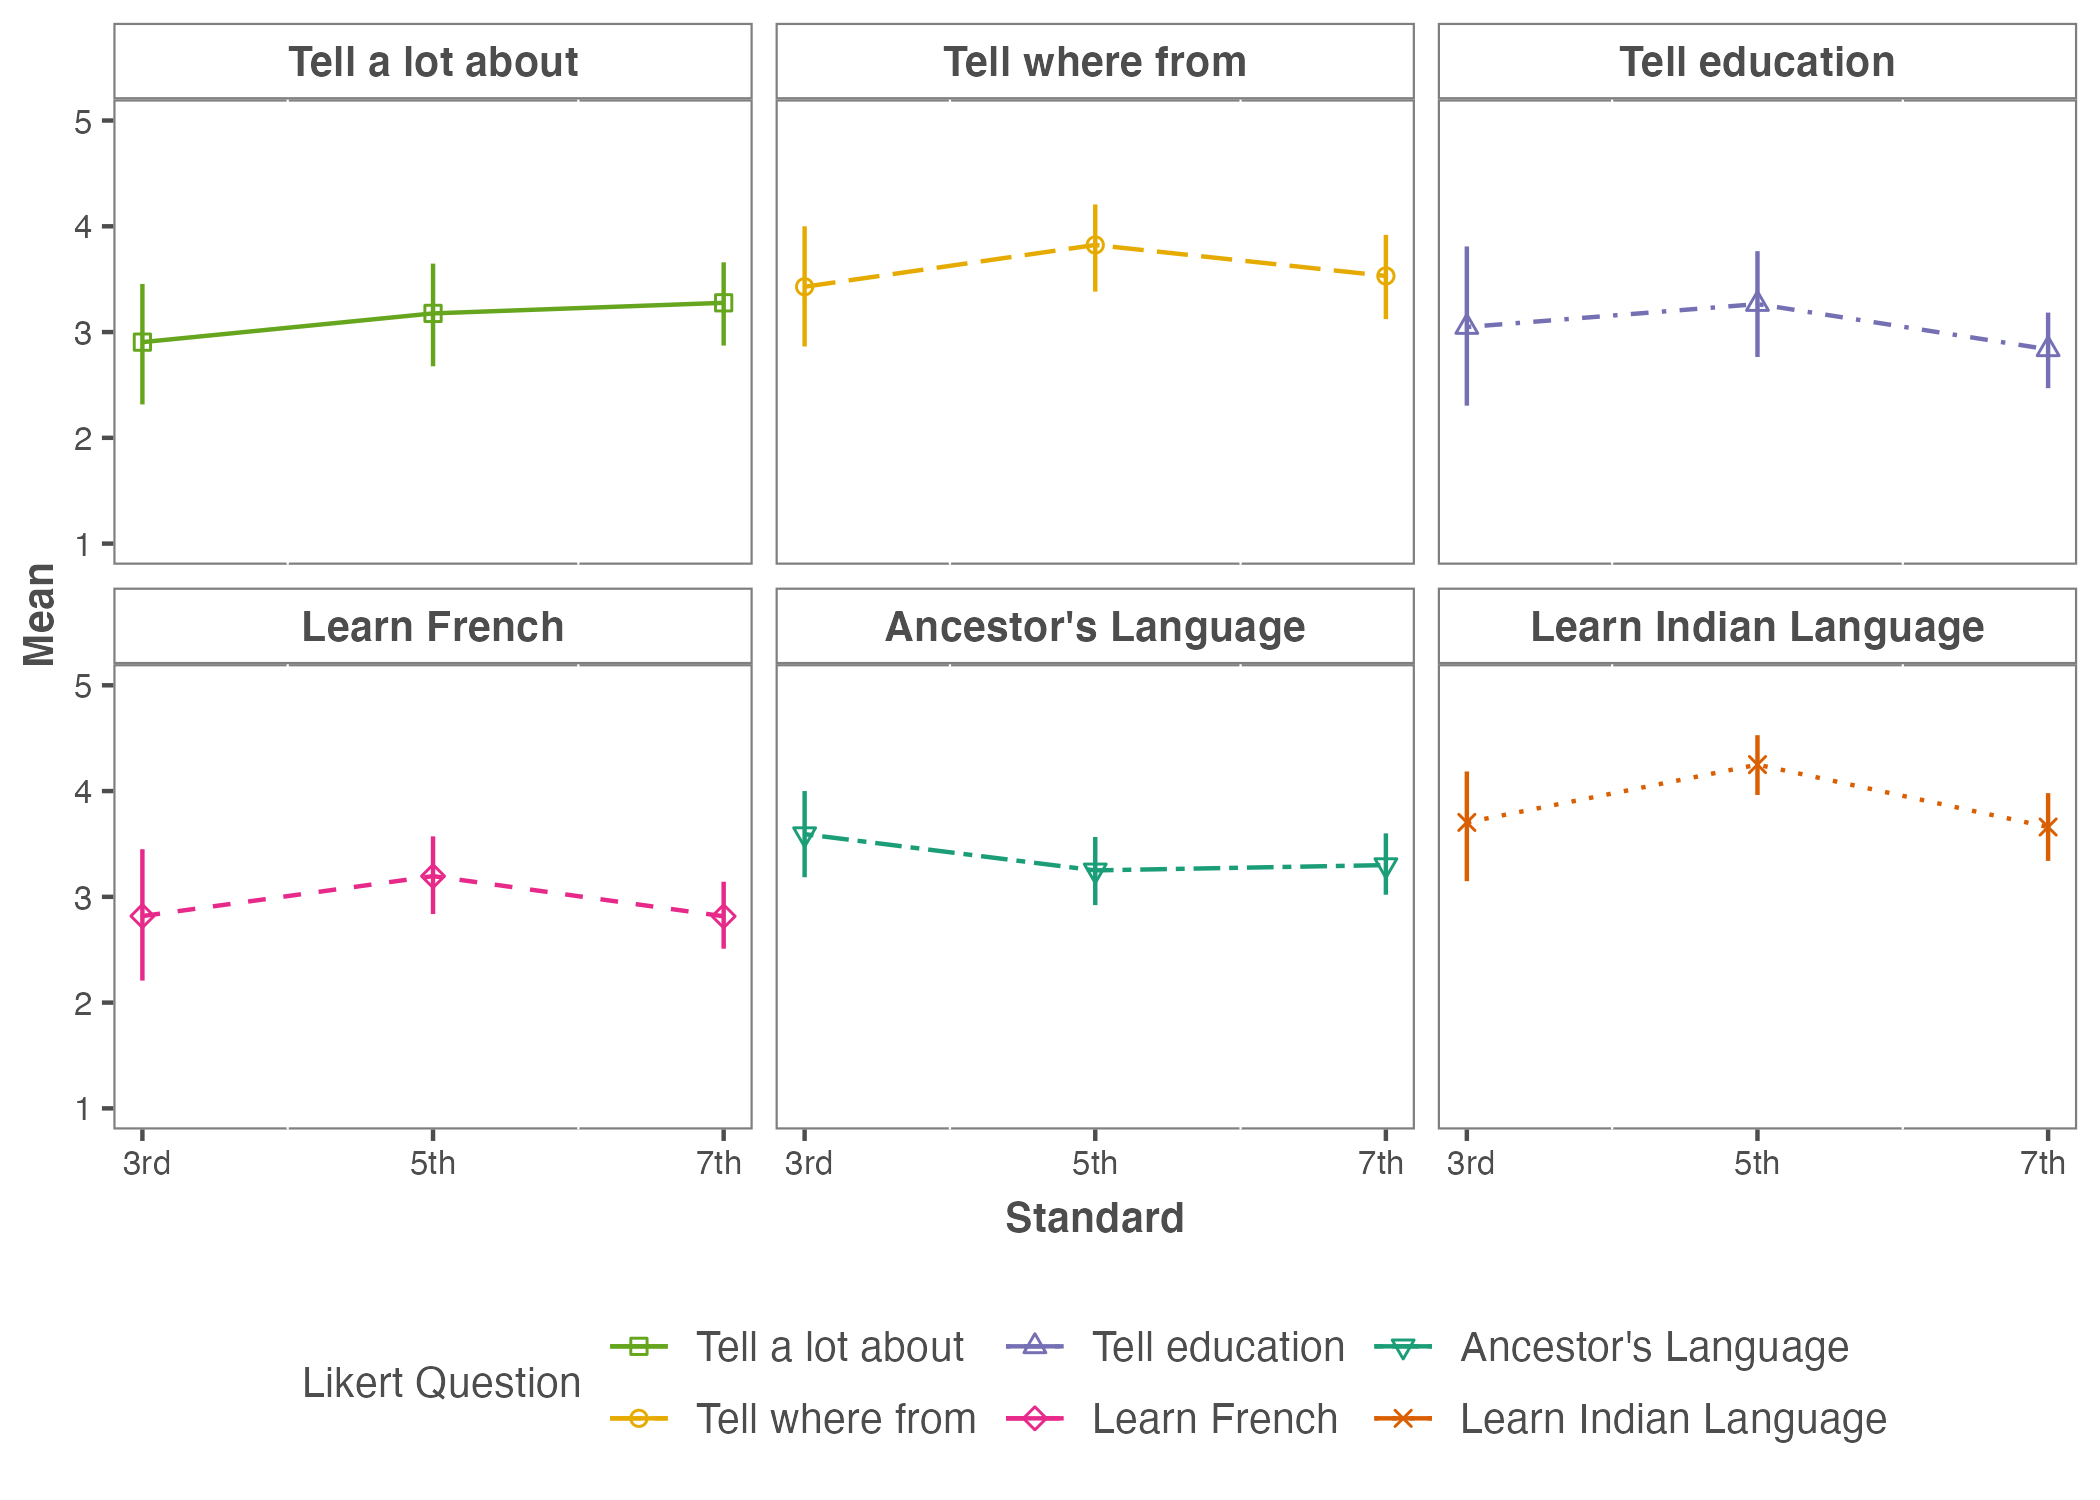
\includegraphics[width=\linewidth]{figures/std_plots/likert_std.png}
    \caption{}
    \label{fig:likert}
\end{figure}